
% Identificar os vários algoritmos, primitivas criptográficas e workflows que garantem a segurança da mDL

\subsection{Controlos de segurança}
\label{sec:orgbc0a271}
\subsubsection{Autenticação Passiva (ISO/IEC 18013-3)}
\label{sec:org479f770}
A autenticação passiva tem como objetivo confirmar que a \emph{machine-readable
data} não foi alterada desde que a IDL (ISO-compliant driving license) foi
emitida.

Na prática, este mecanismo é implementado usando criptografia de chave
pública (assimétrica) para produzir assinaturas digitais sobre
\emph{machine-readable data}.

De facto, se for usado \emph{standard encoding}, a \emph{machina-readable data} deve
incluir:
\begin{itemize}
\item uma \emph{message digest} de cada grupo de dados presente na IDL;
\item uma assinatura digital relativa à coleção de todos as \emph{message digest}. Esta
assinatura deve usar a chave privada da autoridade emissora (IA). (TODO: É
a mesma chave privada para todas as IDL emitidas pela mesma IA?)
\end{itemize}

Posteriormente, quando uma autoridade de leitura (RA) tentar aceder ao
conteúdo da IDL, esta deve realizar os seguintes passos:
\begin{itemize}
\item verificar a assinatura digital utilizando a chave pública da IA.
\item computar o \emph{message digest} para cada um dos grupos de dados que sejam de
interesse e comparar o seu resultado com os respetivos \emph{message digest}
guardados no \emph{machine-readable data} do IDL.
\end{itemize}

Desta forma, após os passos anteriores estarem concluídos, a RA pode
considerar que os grupos de dados que quer ler são autenticos se:
\begin{itemize}
\item a assinatura digital verifica;
\item os \emph{message digest} calculados correspondem aos armazenados na
\emph{machine-readable data};
\item a RA está confiante que a chave pública, usada para verificar a
assinatura, pertence efetivamente à IA que emitiu a IDL.
\end{itemize}

No entanto, caso algum dos passos anteriores não for válido, então significa
que pelo menos um dos seguintes aspetos aconteceu:
\begin{itemize}
\item a assinatura digital não foi verificada com sucesso;
\item a chave pública usada não era a correta;
\item os dados na IDL foram alterados.
\end{itemize}

\begin{enumerate}
\item Funções de Hash
\label{sec:org2a0f02b}
Para \emph{standard encoding} a IA deve utilizar funções de hash presentes na
seguinte lista:
\begin{itemize}
\item SHA-1 (apenas por compatibilidade)
\item SHA-224
\item SHA-256 (recomendada)
\item SHA-384
\item SHA-512
\end{itemize}

Um \emph{message digest} é calculado para cada grupo de dados presente na IDL e
armazenado na \emph{machine-readable data}.

A mesma função de hash deve ser usada para todos os grupos de dados.

O cálculo do \emph{message digest} deve ser aplicado à concatenação de todos os
elementos de dados, presentes num dado grupo de dados, pela ordem
especificada no ISO/IEC 18013-2. (TODO: Ver a ordem)

\item Método de assinatura
\label{sec:org4555f78}
A assinatura digital do IDL deve ser gerada sobre a concatenação dos
\emph{message digest} dos grupos de dados presentes. Para tal, a IA pode utilizar
dois métodos de assinatura diferentes:
\begin{itemize}
\item ECDSA
\item RSA
\end{itemize}

Por um lado, caso a IA opte pelo uso do ECDSA, então deve:
\begin{itemize}
\item usar ANSI X9.62
\item incluir, de forma explícita, na chave pública os parâmetros de domínio da
curva elíptica usados para gerar o par de chaves ECDSA. Assim, esta
informação deve ser do tipo \texttt{ECParameters} (sem nomes de curvas e sem
parâmetros implícitos) e deve incluir o \emph{cofactor} opcional.
\item garantir que os \texttt{ECPoints} estão no formato descompactado.
\item garantir que o tamanho mínimo da ordem do ponto base seja 160 bits.
\end{itemize}

Por outro lado, caso a IA opte pelo uso do RSA, então deve:
\begin{itemize}
\item seguir o RFC 4055, ou seja, escolher o mecanismo RSASSA-PSS (recomendado)
ou o RSASSA-PKCS1-v1\_5.
\item garantir que o tamanho mínimo do \emph{modulus} (n) é 1024 bits. (TODO: o que é
o modulus?)
\end{itemize}

Assim sendo, a IA, além do \texttt{EF.COM} e dos grupos de dados mencionados no
ISO/IEC 18013-2 (TODO: Ver quais são.), deve adicionar um SOD para incluir
as hashes individuais de cada grupo de dados e a assinatura digital no IDL.
O SOD deve ser do tipo \texttt{SignedData} (RFC 3369) e deve ser produzido no
formato DER.

\end{enumerate}

\subsubsection{Autenticação Ativa (ISO/IEC 18013-3)}
\label{sec:org940f982}
A autenticação ativa tem como objetivo confirmar que a \emph{secure integrated
chip} (SIC) foi emitido juntamente com a \emph{machine-readable data}.

O processo a partir do qual esta confirmação é realizada, baseia-se num
protocolo \emph{challenge-response}. Este admite que cada SIC tem um par de chaves.
Por um lado, a chave privada encontra-se armazenada na memória segura do SIC
e não pode ser copiada. Por outro lado, a chave pública é armazenada no
grupo de dados DG13, no formato da estrutura \texttt{SubjectPublicKeyInfo} (RFC 3280)
e deve ser produzido no seguinte formato \texttt{DER}:

\begin{center}
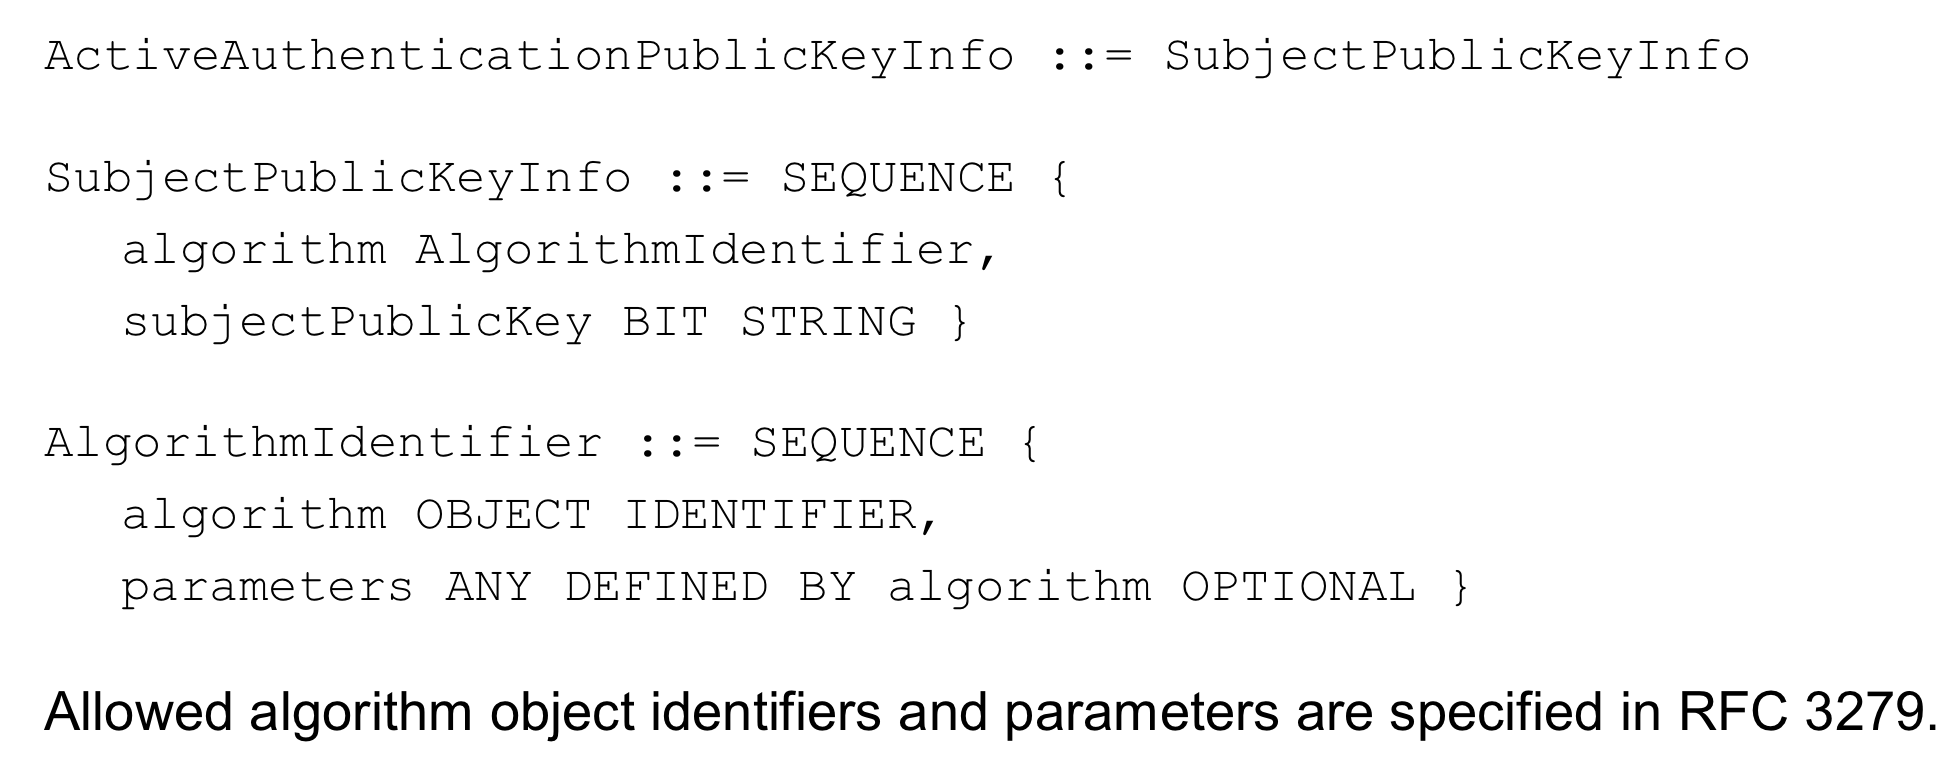
\includegraphics[width=.9\linewidth]{./images/subjectPublicKeyInfo_der.jpeg}
\end{center}

Na prática, o sistema de inspeção (IS) que quiser validar a autenticidade do
SIC deverá criar um desafio escolhido aleatoriamente e enviar ao SIC para
que este o assine com a chave privada e devolva o resultado. Posteriormente,
o IS valida a assinatura com a chave pública do SIC. Se a assinatura for
válida então o SIC foi emitido juntamente com a \emph{machine-readable data}.

O algoritmo do desafio deve respeitar o comando ISO7816 INTERAL AUTHENTICATE
como definido no ISO/IEC 7816-4:2005. O desafio em si deve corresponder a um
\texttt{nonce} (RND.IFD) de 8 bytes de comprimento. (TODO: esta descrição corresponde
ao que está no ISO anterior?)

A geração da assinatura por parte do SIC deve usar um dos seguintes métodos:
\begin{itemize}
\item RSA
\item ECC
\end{itemize}

No caso do primeiro, a assinatura deve respeitar o ISO 9796-2 Digital
Signature Scheme 1. O M deve ser composto por um nonce de c-4 bits (gerado
pelo SIC) e por um RND.IFD (TODO: o que é isto?). Deve ser usado o SHA-1 e o
\emph{trailer option 1}. O resultado da geração da assinatura deverá ser a
assinatura \(\Sigma\), sem a parte da mensagem recuperável M2.

No caso do ECC, a assinatura deve respeitar o ANSI X9.62 ECDSA. O SHA-1 deve
ser usado como algoritmo de hash e o resultado da geração da assinatura deve
ser um DER com dois inteiros (r e s) codificados em ASN.1:

SEQUENCE ::= \{ r INTEGER, s INTEGER \}

\subsubsection{Proteção de acesso básico (BAP)}
\label{sec:orgd21bd93}
A proteção básica de acesso tem como objetivo verificar que o IS tem acesso
ao \emph{proximity integrated circuit card} (PICC) antes de aceder aos dados
guardados no seu interior. Adicionalmente, o BAP assegura que a comunicação
entre o IS e o PICC é protegida. 

Desta forma, o acesso aos dados por parte do IS só é permitido depois de
este assegurar que tem autorização para o fazer. Para que tal aconteça, este
deve sujeitar-se a um protocolo de \emph{challenge-response}. Na prática, IS prova
que tem conhecimento das chaves de acesso básico aos documentos que
pertencem ao PICC e são derivadas a partir do \emph{input} do desafio.
Consequentemente, é originada uma chave de sessão que permite a existência
de uma comunicação segura (\emph{Secure Messaging}).

(TODO: Mais info? Anexo B da parte 3)

\subsubsection{Proteção de acesso extendido (EAP)}
\label{sec:org6117d54}
A proteção de acesso extendido tem como objetivo permitir o acesso
condicional autenticado a certos grupos de dados.
(TODO: é para falar disto?)
\subsubsection{PACE}
\label{sec:org54755e3}
\begin{itemize}
\item Quando uma \emph{password} de acesso ao mDL não é partilhada por uma interface
de comunicação separada, usa-se um mecanismo que suporte a criação de uma
chave efémera forte (e.g. PACE ou EAC).

Anexo I substitui ISO 18013-3 Anexo C.
(TODO: é para falar disto?)
\end{itemize}

\subsection{Controlos de privacidade}
\label{sec:org1279156}
\subsubsection{Consentimento do utilizador}
\label{sec:orga2915d6}
O acesso, por parte de um dispositivo de leitura, aos dados guardados numa
mDL, apenas deve ser permitido depois do consentimento (implícito ou
explícito) do mDL \emph{holder}.

Os métodos para o consentimento do utilizador não fazem parte dos temas
abrangidos neste documento.

Com o objetivo de proteger a privacidade do mDL \emph{holder}, aplicações do
governo não devem rastrear os movimentos de indivíduos através de \emph{geo
tagging}.

